% shared preamble of the theory figures (white background, purple / black theme, sans-serif)
\documentclass[tikz,border=8pt]{standalone}
\usepackage[T1]{fontenc}
\usepackage[scaled=0.92]{helvet}
\renewcommand{\familydefault}{\sfdefault}
\usepackage{amsmath,amssymb}
\usepackage[helvet]{sfmath}
\usetikzlibrary{arrows.meta,calc,decorations.pathreplacing,positioning,backgrounds}
\definecolor{ink}{HTML}{1A1A1F}
\definecolor{cohesin}{HTML}{6A3DE8}
\definecolor{condensin}{HTML}{1BAF7A}
\definecolor{fwd}{HTML}{D1303F}      % CTCF pointing right
\definecolor{rev}{HTML}{2B62D9}      % CTCF pointing left
\definecolor{panel}{HTML}{F8F6FD}
\definecolor{panelline}{HTML}{E3DDF5}
\tikzset{
  fiber/.style={line width=2.1pt,ink,line cap=round,line join=round},
  halo/.style={line width=6pt,white,line cap=round},
  lab/.style={font=\small,text=ink},
  note/.style={font=\footnotesize,text=ink!60},
  hd/.style={font=\bfseries\small,text=ink,anchor=west},
  leader/.style={line width=0.6pt,ink!45},
}
% soft panel, numbered badge, heading
\newcommand{\panelbg}[4]{\draw[rounded corners=9pt,fill=panel,draw=panelline,line width=0.9pt] (#1,#2) rectangle (#3,#4);}
\newcommand{\badge}[3]{\fill[ink] (#1,#2) circle (0.21);\node[white,font=\bfseries\footnotesize] at (#1,#2) {#3};}
% CTCF: a protein on the fibre carrying an arrow that gives the motif direction (f = right, r = left)
\newcommand{\protf}[2]{\draw[rounded corners=3.5pt,line width=0.6pt,draw=fwd!65!black,fill=fwd] (#1-0.3,#2-0.19) rectangle (#1+0.3,#2+0.19);
  \draw[white,line width=1.5pt,-{Stealth[length=3.4pt,width=4.4pt]}] (#1-0.15,#2)--(#1+0.16,#2);}
\newcommand{\protr}[2]{\draw[rounded corners=3.5pt,line width=0.6pt,draw=rev!65!black,fill=rev] (#1-0.3,#2-0.19) rectangle (#1+0.3,#2+0.19);
  \draw[white,line width=1.5pt,-{Stealth[length=3.4pt,width=4.4pt]}] (#1+0.15,#2)--(#1-0.16,#2);}
\newcommand{\prot}[3]{\csname prot#3\endcsname{#1}{#2}}
% ring seen at an angle, drawn as a tube (dark outline, light core); back half and front half
\newcommand{\ringpart}[5]{\draw[line width=4.6pt,#3!80!black,line cap=round] ([shift={(#1,#2)}]#4:0.55 and 0.21) arc[start angle=#4,end angle=#5,x radius=0.55,y radius=0.21];
  \draw[line width=2.4pt,#3!55!white,line cap=round] ([shift={(#1,#2)}]#4:0.55 and 0.21) arc[start angle=#4,end angle=#5,x radius=0.55,y radius=0.21];}
\newcommand{\ringback}[3]{\ringpart{#1}{#2}{#3}{180}{0}}
\newcommand{\ringfront}[3]{\ringpart{#1}{#2}{#3}{180}{360}}
% smooth loop whose foot (ring) is at (cx,y0): half-width W, height H, ring colour
\newcommand{\lloop}[5]{%
  \ringback{#1}{#2}{#5}%
  \draw[fiber] (#1-0.3,#2) .. controls (#1-0.3,#2+0.25*#4) and (#1-#3,#2+0.2*#4) .. (#1-#3,#2+0.55*#4)
     .. controls (#1-#3,#2+0.95*#4) and (#1-0.5*#3,#2+#4) .. (#1,#2+#4)
     .. controls (#1+0.5*#3,#2+#4) and (#1+#3,#2+0.95*#4) .. (#1+#3,#2+0.55*#4)
     .. controls (#1+#3,#2+0.2*#4) and (#1+0.3,#2+0.25*#4) .. (#1+0.3,#2);%
  \ringfront{#1}{#2}{#5}}
% gently undulating fibre from x0 to the loop foot at cx (height y0), and from x1
\newcommand{\base}[4]{%
  \draw[fiber] plot[smooth] coordinates {(#1,0.05) (#1+0.35*#3-0.35*#1,-0.05) (#3-1.4,0.04)} .. controls (#3-0.6,0.02) and (#3-0.3,0.05) .. (#3-0.3,#4);
  \draw[fiber] plot[smooth] coordinates {(#2,-0.05) (#2-0.35*#2+0.35*#3,0.05) (#3+1.4,-0.04)} .. controls (#3+0.6,-0.02) and (#3+0.3,0.05) .. (#3+0.3,#4);}
% stop sign for a blocked leg and a leg arrow
\newcommand{\stopbar}[3]{\draw[#3,line width=2.4pt,line cap=round] (#1,#2-0.2)--(#1,#2+0.2);}
\newcommand{\legarrow}[3]{\draw[cohesin,line width=1.6pt,-{Stealth[length=5pt,width=6pt]},line cap=round] (#1,#3)--(#2,#3);}

\tikzset{bead/.style={fill=ink,draw=white,line width=0.5pt},off/.style={draw=cohesin,dash pattern=on 1.6pt off 1.4pt,line width=0.9pt},
  pass/.style={cohesin,line width=2.2pt,line cap=round,line join=round},thin/.style={line width=1.3pt,ink!70}}
% chain of beads i=0..n along x (wavy); beads lo..hi have their excluded volume off (dashed)
\newcommand{\chain}[6]{% x0, dx, y0, n, off-lo, off-hi
  \foreach \i in {0,...,\numexpr#4-1\relax}{\pgfmathsetmacro{\ax}{#1+\i*#2}\pgfmathsetmacro{\ay}{#3+0.17*sin(\i*55)}\pgfmathsetmacro{\bx}{#1+(\i+1)*#2}\pgfmathsetmacro{\by}{#3+0.17*sin((\i+1)*55)}
    \draw[thin] (\ax,\ay)--(\bx,\by);}
  \foreach \i in {0,...,#4}{\pgfmathsetmacro{\ax}{#1+\i*#2}\pgfmathsetmacro{\ay}{#3+0.17*sin(\i*55)}\pgfmathtruncatemacro{\isoff}{(\i>=#5)*(\i<=#6)}
    \ifnum\isoff=1\draw[off] (\ax,\ay) circle (0.13);\else\draw[bead] (\ax,\ay) circle (0.12);\fi}}
% B strand: left end, middle at height v above A, right end (smooth)
\newcommand{\bstrand}[3]{\draw[pass] plot[smooth] coordinates {(#1-1.45,#2+1.0) (#1-0.75,#2+0.45) (#1,#2+#3) (#1+0.75,#2+0.45) (#1+1.45,#2+1.0)};}
% A strand of 11 beads centred at cx; dashed (EV off) beads 3..7 when off=1
\newcommand{\astrand}[3]{\foreach \i in {0,...,9}{\pgfmathsetmacro{\ax}{#1+(\i-5)*0.3}\pgfmathsetmacro{\bx}{#1+(\i-4)*0.3}\draw[thin] (\ax,#2)--(\bx,#2);}
  \foreach \i in {0,...,10}{\pgfmathsetmacro{\ax}{#1+(\i-5)*0.3}\pgfmathtruncatemacro{\isoff}{#3*(\i>=3)*(\i<=7)}
    \ifnum\isoff=1\draw[off] (\ax,#2) circle (0.11);\else\draw[bead] (\ax,#2) circle (0.1);\fi}}
\begin{document}
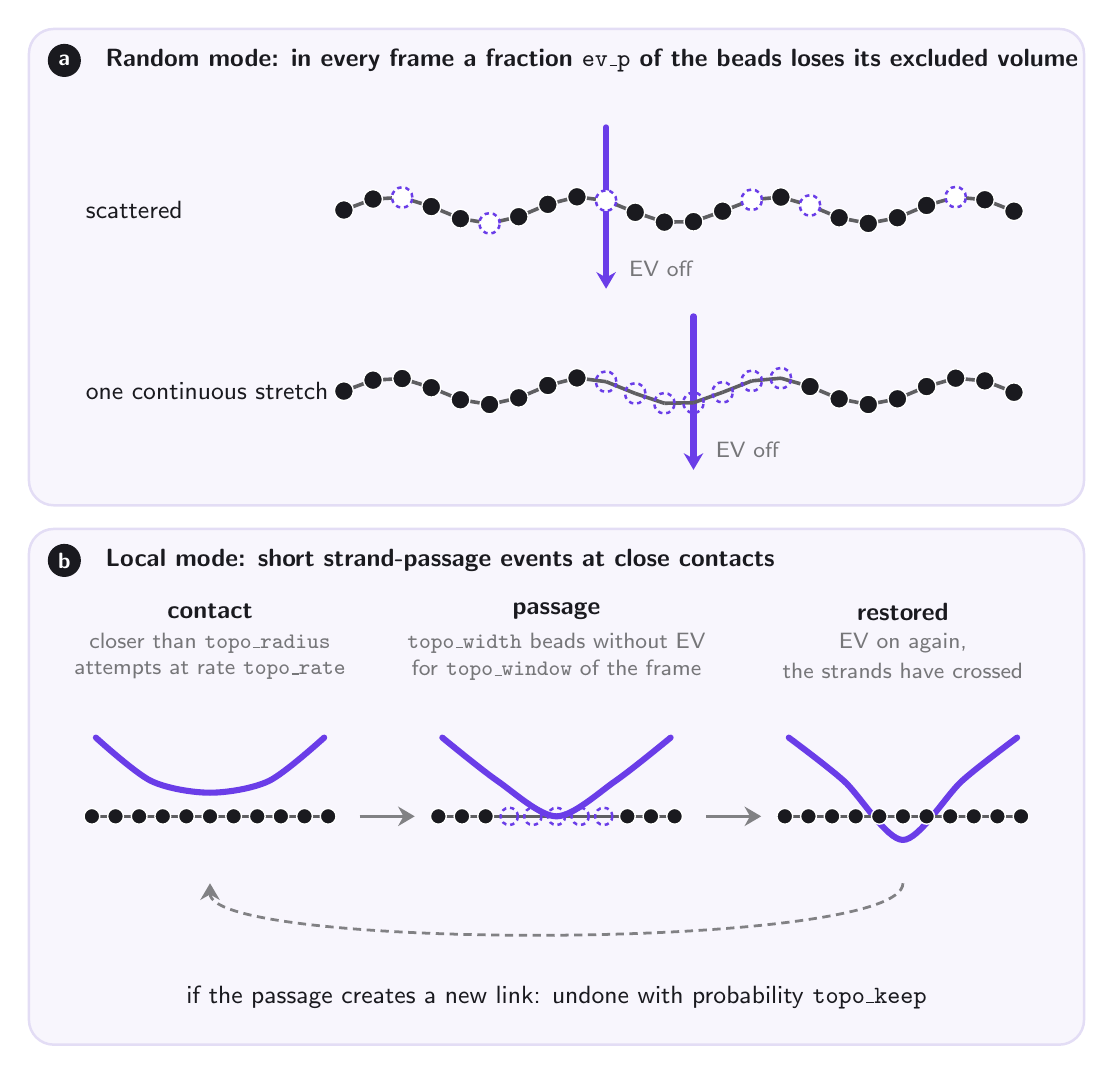
\begin{tikzpicture}
  \panelbg{0}{-5.75}{13.4}{0.3}\panelbg{0}{-12.6}{13.4}{-6.05}
  % a: random mode
  \badge{0.45}{-0.1}{a}\node[hd] at (0.85,-0.1) {Random mode: in every frame a fraction \texttt{ev\_p} of the beads loses its excluded volume};
  \node[lab,anchor=west] at (0.6,-2.0) {scattered};\node[lab,anchor=west] at (0.6,-4.3) {one continuous stretch};
  \draw[pass,-{Stealth[length=6pt,width=7pt]}] (7.33,-0.95)--(7.33,-3.0);      % strand passing through bead 9 of row 1 (x = 4.0 + 9 * 0.36 + ...)
  \chain{4.0}{0.37}{-2.0}{23}{99}{-1}
  \foreach \i in {2,5,9,14,16,21}{\pgfmathsetmacro{\ax}{4.0+\i*0.37}\pgfmathsetmacro{\ay}{-2.0+0.17*sin(\i*55)}\draw[off,fill=white] (\ax,\ay) circle (0.13);}
  \draw[pass,-{Stealth[length=6pt,width=7pt]}] (8.44,-3.35)--(8.44,-5.3);
  \chain{4.0}{0.37}{-4.3}{23}{9}{15}
  \node[note,anchor=west] at (7.5,-2.75) {EV off};\node[note,anchor=west] at (8.6,-5.05) {EV off};
  % b: local mode
  \badge{0.45}{-6.45}{b}\node[hd] at (0.85,-6.45) {Local mode: short strand-passage events at close contacts};
  \foreach \cx/\t/\u/\w in {2.3/contact/{closer than \texttt{topo\_radius}}/{attempts at rate \texttt{topo\_rate}},6.7/passage/{\texttt{topo\_width} beads without EV}/{for \texttt{topo\_window} of the frame},11.1/restored/{EV on again,}/{the strands have crossed}}{
    \node[lab,font=\bfseries\small] at (\cx,-7.1) {\t};\node[note] at (\cx,-7.5) {\u};\node[note] at (\cx,-7.85) {\w};}
  \astrand{2.3}{-9.7}{0}\bstrand{2.3}{-9.7}{0.3}\astrand{6.7}{-9.7}{1}\bstrand{6.7}{-9.7}{0}\bstrand{11.1}{-9.7}{-0.3}\astrand{11.1}{-9.7}{0}
  \draw[-{Stealth[length=6pt,width=7pt]},ink!55,line width=1pt] (4.2,-9.7)--(4.9,-9.7);\draw[-{Stealth[length=6pt,width=7pt]},ink!55,line width=1pt] (8.6,-9.7)--(9.3,-9.7);
  \draw[-{Stealth[length=6pt,width=7pt]},ink!55,line width=1pt,dash pattern=on 3pt off 2pt] (11.1,-10.55) to[out=-90,in=-90,looseness=0.25] (2.3,-10.55);
  \node[lab,fill=panel,inner sep=2pt] at (6.7,-12.0) {if the passage creates a new link: undone with probability \texttt{topo\_keep}};
\end{tikzpicture}
\end{document}
